% !Mode:: "TeX::UTF-8"
\documentclass[slovensky]{svk}
\usepackage[round]{natbib}
\usepackage{subfig}
\usepackage{array}

\begin{document}
  \catcode`\"=\active \def "{\begingroup\clqq\def "{\endgroup\crqq}}

\title{Gnarley Trees}

\author{
  Katka Kotrlová % \email{katkin email, ktorý chce zverejniť}
  \and 
  Pavol Lukča % \email{palyho mail}
  \and
  Viktor Tomkovič % \email{viktor.tomkovic@gmail.com}
  \and 
  Tatiana Tóthová % \email{táničkin mail}
}

\supervisor{
  Jakub Kováč %\email{kuko@ksp.sk}
  \email{algvis@googlegroups.com}
}

%% nasleduje kratka verzia nazvu clanku a 
%% zoznam autorov (bez krstnych mien)
%% tieto informacie sa zobrazuju v hlavicke
\titlerunning{Gnarley Trees}
\authorrunning{Kotrlová, Lukča, Tomkovič, Tóthová}

\institute{
Katedra informatiky,
FMFI UK,
Mlynská Dolina,
842~48~Bratislava}

\maketitle

\begin{abstract}
V tomto článku prezentujeme našu prácu na projekte Gnarley Trees, ktorý 
začal Jakub Kováč ako svoju bakalársku prácu. Gnarley Trees je 
projekt, ktorý má dve časti. Prvá časť sa zaoberá kompiláciou dátových 
štruktúr, ktoré majú stromovú štruktúru, ich popisom a popisom ich 
hlavných výhod a nevýhod oproti iným dátovým štruktúram. Druhá časť sa 
zaoberá ich vizualizáciou a vizualizáciou vybraných algoritmoch na 
týchto štruktúrach.

\noindent
\textbf{Dostupnosť:} Softvér je voľne dostupný na stránke
                     \url{people.ksp.sk/~kuko/gnarley-trees}.
\keywords{Gnarley Trees, vizualizácia, algoritmy a dátové štruktúry}
\end{abstract}

\section{Úvod}
Ako ľudia so záujmom o dátové štruktúry sme sa rozhodli pomôcť vybudovať 
dobrý softvér na vizualizáciu algoritmov a dátových štruktúr a obohatiť 
kompiláciu Jakuba Kováča \cite{kuko} o ďalšie dátové štruktúry. 
Vizualizujeme rôznorodé dátové štruktúry. Z binárnych vyvažovaných stromov 
to sú \emph{finger tree} a \emph{reversal tree}, z háld to sú \emph{d-nárna 
halda}, \emph{ľavicová halda}, \emph{skew halda} a \emph{párovacia halda}. 
Taktiež vizualizujeme aj \emph{problém disjuktných množín (union-find 
problém)} pomocou grafov a \emph{písmenkový strom (trie)}. 

Okrem vizualizácie prerábame softvér, doplnili sme ho o históriu krokov 
a operácií, jednoduchšie ovládanie a veľa iných vecí, zlepšujúcich 
celkový dojem. Softvér je celý v slovenčine a angličtine a je 
implementovaný v jazyku \texttt{Java}.

\subsection{Vizualizácia}
Dátové štruktúry a algoritmy tvoria základnú, prvotnú časť výučby 
informatiky. Vizualizácia algoritmov a dátových štruktúr je grafické 
znázornenie, ktoré abstrahuje spôsob ako algoritmus a dátové štruktúry 
pracujú od ich vnútornej reprezentácie a umiestnení v pamäti. Je teda 
vyhľadávaná a všeobecne rozšírená pomôcka pri výučbe. Výsledky výskumov 
ohľadne jej efektívnosti sa líšia, od stavu \uv{nezaznamenali sme výrazné 
zlepšenie} po \uv{je viditeľné zlepšenie}. \cite{shaffer}

Rozmach vizualizačných algoritmov priniesla najmä Java a jej fungovanie 
bez viazanosti na konkrétny operačný systém. Kvalita vizualizácií sa líši 
a keďže ide o ľahko naprogramovateľné programy, je ich veľa a sú pomerne 
nekvalitné. V takomto množstve je ťažké nájsť kvalitné vizualizácie. 
Zbieraním a analyzovaním kvality sa venuje skupina AlgoViz, ktorá už 
veľa rokov funguje na portále \url{http://algoviz.org/}.

Zaujímavé je pozorovanie, že určovanie si vlastného tempa pri vizualizácií 
je veľká pomôcka. Naopak, ukazovanie pseudokódu alebo nemožnosť určenia si
vlastného tempa (napríklad animácia bez možnosti pozastavenia), takmer 
žiadne zlepšenie neprináša. \cite{shaffer,saraiya}

\subsection*{Motivácia}
Z vyššie uvedeného je jasné, že našou snahou je vytvoriť kvalitnú kompiláciu 
a softvér, ktorý bude nezávislý od operačného systému, bude vyhovovať ako 
pomôcka pri výučbe ako aj pri samoštúdiu a bude voľne prístupný a náležite 
propagovaný. Toto sú hlavné body, ktoré nespĺňa žiaden slovenský a 
len veľmi málo svetových vizualizačných softvérov. Našou hlavnou snahou 
je teda ponúknuť plnohodnotné prostredie pri učení.
%co robime? na co je dobra vizualizacia? (mozete porovnat svet s a bez vizualizacie :))
%co konkretne vizualizujeme? preco to robime? (uz daco take je? [da sa odcitovat shaffer])
%
%Friker, makaj! Zvyšok, pomôž!
\section{Rozšírenie predošlej práce}
jednotlive vizualizacie a implementovane ficurie
co sa zmenilo od bakalarky? zoomovanie, komentare, tree layouty, historia a nove ds

Projekt Gnarley Trees sme rozšírili nielen o vizualizácie ďalších dátových
štruktúr, ale pribudli aj softvérové (vizualizačné) vylepšenia.


\def\ins{$\mathop{insert}(x)$}
\def\find{$\mathop{find}(x)$}
\def\delete{$\mathop{delete}(x)$}
\def\reverse{$\mathop{reverse}(i, j)$}
\def\Bp{$\hbox{\rm B}^+$}

\section{Vyvážené stromy}

Pôvodná verzia \citep{kuko} obsahovala vizualizáciu viacerých vyvážených stromov.
K nim sme pridali \Bp-stromy, stromy s prstom a stromy s reverzami.

\subsection{B$^+$-strom}

\paragraph{Popis.}
\emph{\Bp-strom} je variácia B-stromu, v ktorom sú všetky kľúče uložené v listoch
a listy sú pospájané do spájaného zoznamu. \Bp-strom rádu $B$ je strom, v ktorom
má každý vnútorný vrchol najmenej $\lfloor B/2 \rfloor$, ale najviac $B$ synov.
Vďaka tomu je dobre vyvážený a jeho operácie sú vykonávané v logaritmickom čase.
\Bp-strom je \emph{asociatívne pole (slovník)}, čiže poskytuje tieto tri operácie:
\begin{itemize}
\item $\mathop{\mathit{insert}}(x)$ -- pridá do stromu $x$;
\item $\mathop{\mathit{find}}(x)$ -- zistí, či sa v strome nachádza $x$;
\item $\mathop{\mathit{delete}}(x)$ -- odstráni zo stromu $x$.
\end{itemize}

Operácia \find\ začne v koreni, nájde v ňom prvý kľúč väčší od hľadaného.
Nech je $i$-ty v poradí, potom hľadanie pokračuje v $i$-tom synovi tohto vrcholu.
Je zrejmé, že ak sa väčší kľúč nenájde, presunieme sa do posledného, $B$-tého syna.
V liste sa už len skontroluje, či sa v ňom hľadaný kľúč nachádza.

Definujeme dve operácie: {\sc Copy-Up} a {\sc Push-Up}, ktoré používa operácia \ins.
Ak má vrchol viac prvkov, ako je maximálny limit, treba ho zmenšiť. Rozdelí sa na dve časti.
Ak vrchol nie je listom, použije sa {\sc Push-Up}, najmenší kľúč pravej časti sa vyberie
a stane sa otcom vytvorených dvoch častí. Pokiaľ to list je, kľúč v ňom musí zostať,
preto sa iba skopíruje. Táto operácia sa nazýva {\sc Copy-Up}.

Operácia \ins\ najprv pomocou operácie \find\ zistí, či štruktúra daný kľúč obsahuje.
Ak nie, je zrejmé, že patrí práve do vrchola, kde \find\ skončil. Ak má vrchol po vložení
viac kľúčov ako maximálny limit, je treba ho zmenšiť. Pokiaľ otcovský vrchol má syna,
do ktorého je možné kľúč presunúť a zároveň syn susedí s veľkým vrcholom, postup je nasledovný.
Nech je vrchol vľavo menší a terajší vrchol je $i$-ty syn v poradí. Potom algoritmus z neho
vyberie najmenší kľúč, presunie ho na miesto $(i-1)$-ho kľúča v otcovskom vrchole. Vymenený
kľúč následne vloží do $(i-1)$-ho syna. Ak sú susedné vrcholy príliš veľké na presun kľúča,
použije sa operácia {\sc Copy-Up}. Nový vrchol s jedným kľúčom, ktorý vznikol, vložíme do
otcovského vrcholu. Ak otcovský vrchol presiahol najväčšiu možnú veľkosť, znova sa aplikuje
popísaný algoritmus s jedným rozdielom -- namiesto {\sc Copy-Up} sa použije {\sc Push-Up}.

Operácia \delete\ najprv pomocou \find\ nájde kľúč, potom ho z vrcholu odstráni. Tento vrchol
môže mať po odstránení menší počet kľúčov ako minimálny limit. Vtedy, ak sa dá, sa prenesie
jeden kľúč zo súrodenca. Ak sa nedá, vrchol sa s ním zlúči. Zároveň sa k nim pridá aj kľúč
z otcovského vrcholu, ktorý ich rozdeľoval. Pokiaľ to spôsobilo, že otcovský vrchol má menej
kľúčov, ako je povolené, znova sa aplikuje predošlý algoritmus. Keďže na koreň sa nevzťahuje
minimálny limit, po skončení bude strom zaručene v konzistentnom tvare.

%\paragraph{Časová zložitosť}
%\todo{toto je pocet pristupov na disk! pocet krokov je $O(B\log_B n)$; ale pocet pristupov
%na disk nas zaujima, lebo disk je pomaly}
Vkladanie, vymazávanie a hľadanie má časovú zložitosť $O(\log_B n)$.

\paragraph{Použitie.}
Hlavné využitie \Bp-stromov je v databázových systémoch. Ak zvolíme vhodný rád, vieme jednotlivé
vrcholy dobre napasovať na stránky a tým regulovať ako počet prístupov k pamäti, tak jej zaplnenie
\citet{sahni}. Agregačné funkcie, ako napríklad súčet, minimum, priemer, vieme pre daný interval
spočítať v čase $O(\log_B(n))$. Vypísať všetky prvky z daného intervalu dokážeme pomocou
$O(\log_B(n) + t/B)$ prístupov na disk.
% \Bp-strom podporuje efektívne vyhľadanie prvkov poľa, ktoré patria do daného intervalu.
% Algoritmus nájde jeden krajný bod a vďaka spájanému zoznamu, vytvorenému z listov, ostatné prvky
% postupne prečíta. Zložitosť je $O(\log_B(n) + t/B)$, kde $t$ je počet výsledných kľúčov z hľadaného intervalu.

Ďaľšia výhoda \Bp-stromov oproti B-stromom sa prejaví, ak máme utriedený zoznam dát a chceme z neho vytvoriť \Bp-strom:
\Bp-strom môžeme vystavať odspodu. Takýto postup nám zaručí vyžaduje $O((n/B)\cdot\log_B n)$ prístupov na disk,
čo je $B$-krát rýchlejšie ako spraviť $n$ volaní \ins.




\subsection{Strom s prstom}
\emph{Strom s prstom} (z anglického Finger tree) je vyhľadávací strom s hranami na vrstvách a štruktúrou 
nazývanou prst. Prst je smerník na konkrétny vrchol a umožňuje (aj vďaka väzbám navyše) efektívnejší 
prístup k vrcholom v jeho blízkom okolí.

\paragraph{Popis.}
Strom s prstom je upravený 2-3-4$^+$ strom (\Bp-strom rádu 4, t.j.\ vnútorné vrcholy
majú stupeň 2, 3 alebo 4). Kľúče sú uložené v listoch a vnútorné vrcholy
obsahujú ich kópie, aby viedli vyhľadávanie. Pre podporu vyhľadávania
s prstom spojíme všetky vrcholy na rovnakej úrovni (v rovnakej vzdialenosti od koreňa)
do obojsmerného spájaného zoznamu.
Ak sú nejaké dva vrcholy spojené takouto hranou, budeme hovoriť, že sú susedia.

Prst, ako už bolo spomenuté, ukazuje na nejaký vrchol. Môže sa pohybovať po všetkých hranách
a pomocou neho sa vykonávajú všetky operácie. Keďže sú všetky kľúče uložené v listoch, prst
na tejto vrstve začína, aj končí.

Vzhľadom na usporiadanie budem predpokladať, že menšie prvky sa nachádzajú vždy vľavo a každý
prekopírovaný kľúč má svoj originál vždy vľavo v listovom vrchole.

% Strom s prstom je \emph{asociatívne pole (slovník)}, čiže
% poskytuje tieto tri operácie:
% \begin{itemize}
% \item $\mathop{\mathbf{insert}}(\k)$ -- pridá do stromu $\k$;
% \item $\mathop{\mathbf{find}}(\k)$ -- zistí, či sa v strome nachádza $\k$;
% \item $\mathop{\mathbf{delete}}(\k)$ -- odstráni zo stromu $\k$.
% \end{itemize}

Operácia \find\ začne na mieste, kam ukazuje prst. Skontroluje, či by kľúč mal patriť do daného
vrcholu. Ak nie, pozrie sa, či nepatrí do niektorého zo susedov. Ak áno, prst sa tam presunie
a vyhľadávanie sa skončilo. Inak smerník prejde o vrstvu vyššie, na otcovský vrchol. Ak hľadaný
kľúč patrí do jeho podstromu (t.j.\ je väčší ako jeho najmenší kľúč a menší ako ten najväčší),
zíde po hranách do listu, kde by sa daný kľúč mal nachádzať. Keď do podstromu nepatrí, skontroluje,
či nepatrí do podstromu susedov. Ak áno, prejde po vrstevnej hrane na suseda a následne zíde až
do listu, kde by mal kľúč byť. Pokiaľ prst nenarazil na správny podstrom, znova sa presunie smerom
nahor po otcovskej hrane. Hľadanie pokračuje analogicky. Je zrejmé, že ak prst ukazuje na koreň,
kľúč bude patriť do jeho podstromu.

% Otázka patričnosti do podstromu sa dá pre krajné prípady optimalizovať. Ak totiž vrchol, na ktorý
% ukazujeme, nemá napríklad pravého suseda, je zrejmé, že vačší kľúč ako je najvačší v tomto vrchole
% v strome nie je. Preto ľubovoľný kľúč do podstromu tohto vrchola patrí práve vtedy, keď je väčší
% ako jeho najmenší prvok. Analogicky to platí, ak chýba ľavý sused.

Operácia \ins\ najprv pomocou operácie \find\ nájde miesto, kam by mal vkladaný kľúč patriť.
Ak taký kľúč už v strome je, ďalší sa nevloží. V prípade, že sme vložili nový kľúč, môže sa stať,
že vrchol "pretečie", tzn.\ má viac ako 3 prvky. Situácia sa vyrieši rovnako ako v \Bp-strome.
Operácia \delete\ najprv pomocou operácie \find\ nájde miesto, kam by mal hľadaný kľúč patriť.
Ak tam nie je, vymazávanie sa končí. Inak sa vymaže. Môže sa stať, že vrchol "podtečie", tzn.\ 
nemá kľúč. Tento problém sa rieši rovnako ako v \Bp-strome.

\paragraph{Časová zložitosť.}
Keďže každý vrchol má aspoň dvoch synov, 2-3-4 strom má hĺbku $O(\log n)$, kde $n$ je počet kľúčov,
a teda podporuje vykonávanie operácií v čase $O(\log n)$. Ak sa však použije prst, časová zložitosť
vychádza na $O(\log d)$, kde $d$ je vzdialenosť pozície prsta a vrcholu, kam patrí cieľový kľúč,
amortizovane dokonca na $O(1)$ \citet{sahni}.

% \paragraph{Použitie.}
% Prst ako smerník na prvok štruktúry, ktorý umožňuje efektívnejší prístup k okolitým kľúčom, prvýkrát
% spomenuli Guibas et al. Vo svojej publikácii prezentujú B-strom podporujúci vyhľadávanie v $O(\log n)$
% a update-y dokonca v $O(1)$ čase, predpokladajúc, že je udržiavaných len $O(1)$ pohyblivých prstov \citet{sahni}.
% Pohyb prsta o $d$ pozícií trvalo $O(\log n)$ času. Na základe tejto práce navrhli Huddleston a Mehlhorn
% svoj vrstvovo spájaný 2-3-4 strom, ktorý bol neskôr upravený vďaka Belloch et al. na priestorovo efektívnejšiu
% alternatívu. Toto riešenie využíva jeden prst, s ktorým štruktúra ponúka rovnakú operačnú zložitosť ako 2-3-4 stromy.
% %Model bol dokonca zovšeobecnený na ($a$,$b$)-stromy, kde $b\geq 2a$.
% %Je zaujímavé, že pre 2-3 strom bola nájdená postupnosť vkladaní a vymazávaní, ktorá vyžaduje $\Omega(n\log n)$ krokov \citet{sahni}.

\paragraph{Vizualizácia.}
Strom s prstom je vizualizovaný pomocou \Bp-stromu s rádom 4, keďže jeho podmienky pre počet potomkov vyhovujú
danej štruktúre.
% Prst je samostaný pohyblivý článok, ktorý si pamätá iba vrchol, na ktorý ukazuje. Po stromovitej
% štruktúre sa vie hýbať vďaka informáciám získaným z daného vrcholu.
\todo{OBRAZOK}



\def\find{$\mathop{find}(k)$}

\subsection{Strom s reverzami}
\emph{Strom s reverzami} je dátová štruktúra na uchovávanie permutácií.
Poskytuje operácie
\begin{itemize}
% \item $\mathop{\mathit{insert}}(\k)$ -- pridá do stromu $\k$;
\item $\mathop{\mathit{find}}(k)$ -- zistí, ktorý prvok je na $k$-tom mieste permutácie;
\item $\mathop{\mathit{reverse}}(i,j)$ -- spraví reverz intervalu od $i$ po $j$.
\end{itemize}

\paragraph{Popis.}
Permutáciu reprezentujeme ako strom, v ktorom je in-order poradie prvkov totožné
s poradím prvkov v permutácií. Strom s reverzami môžeme implementovať pomocou ľubovoľného
vyváženého stromu, ktorý podporuje rozdelenie a zreťazenie dvoch stromov v logaritmickom čase.
My sme zvolili splay strom pre jeho jednoduchosť.

% Splay strom je štruktúrou binárny strom,
% líši sa od neho iba operáciami. Keď pracuje s ľubovoľným prvkom, na konci operácie bude vo vrchole
% buď daný kľúč alebo najbližší z jeho okoli. Na rozdiel od splay stromu, strom s reverzami nepracuje
% s kľúčmi, ale s poradím prvkov. Preto je nutné, aby mal

Aby sme vedeli efektívne vyhľadať $k$-ty prvok, budeme si pre každý vrchol udržiavať veľkosť jeho
podstromu. V operácií \find\ sa vieme podľa toho rozhodnúť, či sa $k$-ty prvok nachádza v ľavom podstrome,
resp.\ koľký prvok je v pravom podstrome. Po nájdení sa prvok presunie do koreňa pomocou operácie splay.

Operáciu \reverse\ implementujeme lenivo:
strom najskôr rozdelíme na tri časti: $T_1,T_2,T_3$, pričom $T_2$ obsahuje interval od $i$-teho
po $j$-ty prvok, $T_1$ obsahuje začiatok a $T_3$ koniec permutácie. Koreň $T_2$ jednoducho
označíme vlajkou, ktorá bude signalizovať, že podstrom je reverznutý a prvky sú v skutočnosti
v opačnom poradí ako doteraz. Ak už koreň vlajku obsahuje, odstránime ju.
Následne stromy $T_1,T_2,T_3$ opäť spojíme.

Pri takomto riešení musíme ešte upraviť vyhľadávanie a rotácie, aby brali do úvahy vlajky vo vrcholoch.
Najelegantnejšie riešenie je odstrániť vlajku vždy, keď na ňu narazíme:
Danému vrcholu odstránime vlajku, vymeníme mu synov a každému synovi vlajkový bit znegujeme.

Všetky operácie vieme implementovať v rovnakom čase ako operácie v splay tree, t.j.\ amortizovane $O(\log n)$.

\paragraph{Použitie.}
Stromy s reverzami (pôvodne založené na AVL stromoch) navrhli \citet{chrobak}
na efektívnu implementáciu 2-opt heuristiky na riešenie problému obchodného cestujúceho.
Pri 2-opt heuristike sa snažíme reverzovať úseky cesty, kým nenájdeme lokálne minimum.

V bioinformatike sa tieto stromy používajú na triedenie orientovaných permuácií
pomocou reverzov \citep{reversals, reversals2}.

Za povšimnutie stojí fakt, že táto dátová štruktúra podporuje výmenu ľubovoľných dvoch blokov
v logaritmickom čase, keďže túto operáciu vieme odsimulovať pomocou štyroch reverzov.

\paragraph{Vizualizácia.}
Pre lepšiu vizualizáciu sme pridali do stromu nultý a posledný prvok. Tieto prvky
do reverzovateľného intervalu nepatria, majú však zmysel v prípade, ak sa reverzuje
interval, ktorý zahŕňa aspoň jeden okraj. V tom prípade v operácii \reverse\ nezostane
ani $T_1$ ani $T_4$ prázdny. Aby nevznikli problémy s operáciami, za krajné kľúče boli
zvolené hodnoty $0$ a číslo o jedna väčšie od aktuálneho maxima. Zároveň, pre lepšiu
predstavu, bolo pridané pole, v ktorom užívateľ vidí skutočné poradie prvkov, ktoré
zo stromu nie je až tak zjavné. Pole simuluje operácie spolu so stromom, ale tie sú
na ňom vykonávané v lineárnom čase.
\section{Haldy}

V nasledujúcom texte sa budeme zaoberať rôznymi druhmi prioritných front. Popíšeme \emph{$d$-árnu haldu} ako 
základnú modifikáciu binárnej haldy, \emph{ľavicovú haldu} a niektoré druhy samoupravujúcich sa háld, konkrétne 
\emph{skew haldu} a \emph{párovaciu haldu}.
Halda je vo všeobecnosti \emph{zakorenený strom} s vrcholmi obsahujúcimi kľúče reprezentujúce dáta. Dôležitá je 
zakladná podmienka haldy, ak vrchol $p(x)$ je otcom vrcholu $x$, potom
$\hbox{\emph{kľúč}}(p(x)) \leq \hbox{\emph{kľúč}}(x)$\footnote{Bez ujmy na všeobecnosti budeme uvažovať o \emph{min haldách},
teda v koreni sa bude nachádzať najmenší prvok. Podobnými úvahami by sme text mohli rozšíriť o \emph{max haldy}
s najväčším prvkom v koreni.}.

Štandardné operácie, ktoré haldy podporujú, a ktorými sa budeme zaoberať pri každej dátovej štuktúre, sú:
\begin{itemize}
%\item $\mathop{\mathit{createHeap}}$ -- vytvorí prázdnu haldu;
\item $\ins(x)$ -- vloží vrchol s kľúčom $x$;
\item $\mathop{\mathit{findMin}}$ -- vráti minimum, t.j. hodnotu kľúča v koreni;
\item $\mathop{\mathit{deleteMin}}$ -- odstráni vrchol s najmenším kľúčom, t.j.\ koreň;
\item $\dec(v, \Delta)$ -- zníži kľúč vrcholu $v$ o $\Delta\geq0$;
\end{itemize}

Niektoré haldy navyše implementujú operáciu $\meld(i, j)$, ktorá spojí haldu $i$ s haldou $j$.

\input haldy/daryheap.tex
\input haldy/leftist.tex
\input haldy/skewheap.tex
\input haldy/pairheap.tex

\section{Union Find}
Sú problémy, ktoré vyžadujú spájanie objektov do množín a množín navzájom 
a následné určovanie, do ktorej množiny objekt patrí. Od takejto \emph{
dátovej štruktúry pre disjunktné množiny} očakávame, že si bude udržiavať 
jednoznačného \emph{zástupcu} každej množiny a bude poskytovať 
tieto tri oprácie: 
\begin{itemize}
\item \textbf{makeset} -- vytvorí novú množinu s jedným prvkom, ktorý 
nepatrí do žiadnej inej množiny;
\item \textbf{find($x$)} -- nájde zástupcu množiny, v ktorej sa 
prvok $x$ nachádza;
\item \textbf{union($x$, $y$)} -- vytvorí novú množinu, ktorá obsahuje 
všetky prvky v množinách, ktorých zástupcovia sú $x$ a $y$. Tieto 
množiny zmaže. Ďalej vyberie nového zástupcu novej množiny. Pre 
jednoduchosť, táto operácia predpokladá, že $x$ a $y$ sú 
\emph{zástupcovia} množín.
\end{itemize}
Vďaka dvom hlavným operáciam \textbf{find} a \textbf{union} sa na Slovensku 
je táto dátová štruktúra známejšia pod poj\-mom \emph{Union-Find}, ktorý 
používame aj my. 

Na reprezentovanie dátovej štruktúry sme si zvolili štruktúru podobnú 
lesu: každá množina je reprezentovaná stromom a zástupca množiny je koreň. 
Ďalej je dôležité, že ku objektom vieme pristupovať pria\-mo (pole).
Teda, objekty majú svoje \emph{id} a pointer \emph{p($x$)} 
ukazujúci na otca v strome. Pointer zástupcu množiny ukazuje na 
hodnotu \texttt{NULL}.\\
rozne kopresie cesty
citovat Walkerov alg.
\\
Yahoo! Walker, Texas ranger, FTW!

\def\k{w}
%\def\kluc{kľúč}
\def\put{$\mathop{\mathit{insert}}(\k)$}
\def\find{$\mathop{\mathit{find}}(\k)$}
\def\delete{$\mathop{\mathit{delete}}(\k)$}
\def\trie{trie}
\def\uz{\hbox{\tt\$}}

\section{Písmenkový strom}
\emph{Písmenkový strom} reprezentuje množinu slov. Oproti binárnym 
vyhľadávacím stromom je hlavný rozdiel v tom, že kľúče nie sú uložené 
vo vrcholoch, ale samotná poloha v strome určuje kľúč (slovo). 

% My používame ako abecedu veľké znaky anglickej 
% abecedy a ukončovací znak značíme dolárom (\uz).



\paragraph{Popis.}
Písmenkový strom je \emph{zakorenený strom}, v~ktorom každá hrana obsahuje 
práve jeden znak z abecedy alebo \emph{ukončovací znak}. Teda, každá cesta 
z koreňa do listu so znakmi $w_1, w_2, \ldots, w_n, \uz$ prirodzene 
zodpovedá slovu $w=w_1w_2\cdots w_n$. \emph{Ukončovací znak} je ľubovoľný, 
dopredu dohodnutý symbol, ktorý sa v abecede nenachádza (napr. \uz). 

Písmenkový strom je \emph{asociatívne pole (slovník)}, čiže 
poskytuje tieto tri operácie:
\begin{itemize}
\item \put\ -- pridá do stromu slovo $\k$;
\item \find\ -- zistí, či sa v strome slovo $\k$ nachádza;
\item \delete\ -- odstráni zo stromu slovo $\k$.
\end{itemize}
Všetky operácie začínajú v koreni a ku slovu pridávajú ukončovací znak, 
teda pracujú s reťazcom $\k\uz$. 

Operácia \put\ vloží do stromu vstupný reťazec tak, že z reťazca číta znaky 
a prechádza po príslušných hranách. Ak hrana s daným symbolom neexistuje, 
pridá ju (pozri obr.~\ref{img:trieinsert}).

\begin{figure}
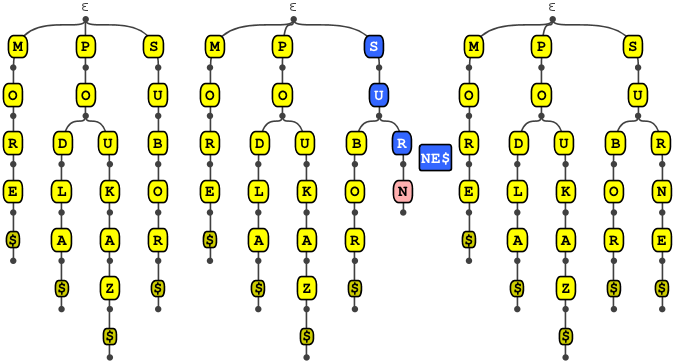
\includegraphics[width=\columnwidth]{obrazky/trieinsertsmall.png}
\caption{\emph{Vloženie slova \uv{{\tt SURNE}}.} Začiatok slova 
\uv{{\tt SU}} sa v strome nachádza, ešte treba pripojiť hrany 
so znakmi {\tt R}, {\tt N}, {\tt E} a \uz.} 
\label{img:trieinsert} 
\end{figure}

Operácia \find\ sa spustí z koreňa podľa postupnosti znakov. Ak hrana, 
po ktorej sa má spustiť neexistuje, dané slovo sa v strome nenachádza. 
Ak prečíta celý vstupný reťazec, dané slovo sa v strome nachádza.

Operácia \delete\ najprv pomocou operácie \find\ zistí umiestnenie slova. 
Ak sa slovo v strome nachádza, algoritmus odstráni hranu s ukončovacím 
znakom a vrchol, ktorý bol na nej zavesený. V tomto štádiu sa nám môže 
stať, že v strome ostane \emph{mŕtva vetva} -- nie je ukončená 
ukončovacím znakom. Pre fungovanie stromu to nevadí, všetky operácie by 
prebiehali správne, ale takto štruktúra zaberá zbytočne veľa miesta. 
Preto je dobré túto mŕtvu vetvu odstrániť (pozri obr.~\ref{img:triedelete}).

\begin{figure}
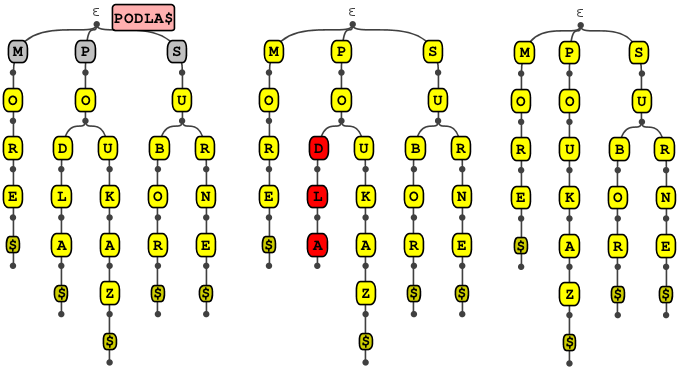
\includegraphics[width=\columnwidth]{obrazky/triedeletesmall.png}
\caption{\emph{Odstránenie slova \uv{{\tt PODLA}}.} Po odstránení 
\uz\ nám v strome ostane nepotrebá prípona \uv{{\tt DLA}} (mŕtva vetva), 
ktorá je vyznačená červenou.}
\label{img:triedelete} 
\end{figure}

\bigskip
% \paragraph{Časová zložitosť.}
Všetky tri operácie majú časovú 
zložitosť $O(|\k|)$, kde $|\k|$ je dĺžka slova.

\paragraph{Použitie.}
Prvýkrát navrhol písmenkový strom \citet{fredkin}, ktorý používal názov 
\emph{trie memory}\footnote{Z anglického re\emph{trie}val -- získanie.}, 
keďže išlo o spôsob udržiavania dát v pamäti. 
%používal operácie 
%$\mathop{storage}$ (\put), $\mathop{retrieval}$ (\find) 
%a $\mathop{deletion}$ (\delete) a dátovú štruktúru nazýval \emph{trie 
%memory}, keďže išlo naozaj o spôsob uloženia dát v pamäti.

%O niečo neskôr \citet{knuth} uviedol vo svojej knihe ako príklad na 
%písmenkový strom vreckový slovník. 
%V tom istom diele uviedol aj možnosť 
%komprimovania vetiev a možnosť prerobenia $m$-árneho \trie\ na binárny. 
%\citet{knuth} však ukázal len komprimovanie koncov vetiev. 
\citet{patricia} navrhol písmenkový strom, v ktorom sa každá cesta bez vetvení
skomprimuje do jedinej hrany (na hranách potom nie sú znaky, ale slová).
Táto štruktúra je známa pod menom \emph{PATRICIA} (tiež \emph{radix tree},
resp.\ \emph{radix trie}) a využíva sa napríklad v \emph{routovacích tabuľkách}
\citep{radix}.

Písmenkový strom (tzv.\ \emph{packed trie} alebo \emph{hash trie}) sa používa
napríklad v programe \TeX\ na slabikovanie slov \citep{liang}.
Pôvodný návrh \citep{fredkin} ako uložiť \trie\ do pamäte zaberal
príliš veľa nevyužitého priestoru. \citet{liang} však navrhol, ako
tieto nároky zmenšiť.

Písmenkové stromy sa podobajú na \emph{konečné automaty}. 
Vznikli rôzne modifikácie stromov na automaty, ktorých hlavnou výhodou je, 
že v komprimovanej podobe spájajú nielen predpony, ale aj prípony slov 
a teda v slovách ľudských jazykov výrazne znižujú pamäťový priestor potrebný 
na uchovanie dátovej štruktúry. Vďaka tomu sa využívajú na jazykovú korekciu, 
automatické dopĺňanie slov a podobne \citep{scrabble,ca}. 

Ďalšie použitie písmenkového stromu je pri triedení zoznamu slov. 
Všetky slová sa pridajú do stromu a potom sa spraví \emph{preorderový prechod} 
stromu. Túto myšlienku spracovali \citet{burstsort1} a veľmi výrazne zrýchlil 
triedenie dlhých zoznamov slov. Neskôr tento algoritmus vylepšili 
\citet{burstsort2}. Kvôli tomu, ako algoritmus pracuje, 
sa nazýva \emph{burstsort}.

% Špeciálnym použitím písmenkového stromu je vytvorenie stromu zo všetkých 
% prípon slova. Táto dátova štruktúra sa nazýva \emph{sufixový strom} a dá sa 
% mo\-di\-fi\-ko\-vať na udržiavanie viacerých slov. Tieto štruktúry majú 
% veľmi veľa praktických využití \citep{gusfield}. 

\paragraph{Vizualizácia.} Pri vizualizácií písmenkového stromu sme použili 
Walkerov algoritumus pre úsporné rozloženie vrcholov v strome
\citep{walker}. Keď má vrchol viacej synov a hrany kreslíme priamo, tak vzniká 
nedostatok priestoru pre umiestnenie znakov na hrany. Preto sme sa rozhodli 
kresliť hrany zakrivene, podľa Bézierovej krivky určenej štyrmi bodmi. 
Vo vizualizácií sa dajú vložiť náhodné slová podľa momentálne nastaveného 
jazyka. Taktiež sa automaticky odstraňuje diakritika a interpunkcia, takže 
sa dá naraz vložiť súvislý text.

\section{História}
ako sme ju do..\\ ..robili.\\
Palyho umelecký opis.
\section{Záver}
work in progress; co sme spravili - uz je v uvode?, preco sme lepsi - sme vobec lepsi (ako galles)?, co este chceme/treba spravit - maybe DONE, co je rozrobene - v podstate to, co chceme spravit - same as previous?
\\
V ďalšej práci sa budeme zaoberať implementovaním ďalších vizualizácií dátových
štruktúr (napríklad "tejto, tejto a aj tejto"), doplnením histórie krokov do
všetkých dátových štruktúr, ale aj vylepšením GUI, refaktorovaním zdrojového
kódu a inými softvérovými vylepšeniami. Našim cieľom je čo najviac zjednodušiť
prácu s programom a tak zefektívniť výučbu jednotlivých dátových štruktúr, resp.
spraviť ju zábavnejšou.


\subsection{Príspevky autorov}
Katka Kotrlová obohatila projekt o vizualizácie d-nárnej, ľavicovej, skew a 
párovacej haldy, Viktor Tomkovič pridal vizualizácie union-findu, písmenkového 
stromu a implementoval algoritmus na vykresľovanie všeobecných stromov, 
Tatiana Tóthová vizualizovala B$^+$-strom, strom s prstom a strom s reverzami 
a Pavol Lukča dorobil históriu krokov a operácií do takmer všetkých slovníkov 
a venoval sa refaktorovaniu zdrojového kódu. Na príprave tohto textu sa 
podieľali všetci autori.


\section*{Poďakovanie}
Autori by sa chceli poďakovať školiteľovi za veľa dobrých rád 
a odborné vedenie pri práci.



\nocite{*}
\bibliographystyle{apalike}
\bibliography{references}

%% citacie ulozte do suboru references.bib
%% na populaciu zoznamu literatury pouzite program
%%
%% bibtex references
%%
%% po ktorom je potrebne dokument znova zlatexovat

\end{document}
